% Intro
The solution must therefore be to implement a (preferably distributed) database on the user side, which means that there is no single authoritative source.
Since the aim is to defend against \emph{targeted} attacks, the assumption being that only few users will encounter a malicious version, this can be circumnavigated by checking the hash against a \emph{consensus} formed by many users.

To make the database as safe as possible, a blockchain is used. The chain contains a smart contract providing securely callable functions. With one of these functions it is possible to commit a hash for a package and version. This hash will be saved in the blockchain only if this user has not committed the same hash before, thereby making it harder to take over the blockchain and get a malicious hash to be the consensus. The consensus is updated after every hash commit. Another function is used to get the current consensus hash and its number of commits for a specific package and version.

This is the first project to use a blockchain as a means to provide distributed verification of (software) downloads.

% Workflow
\subsection*{Workflow}
\label{sec:workflow}
The following workflow is visualized in Figure \ref{fig:main_workflow}.
\begin{figure}
	\centering
		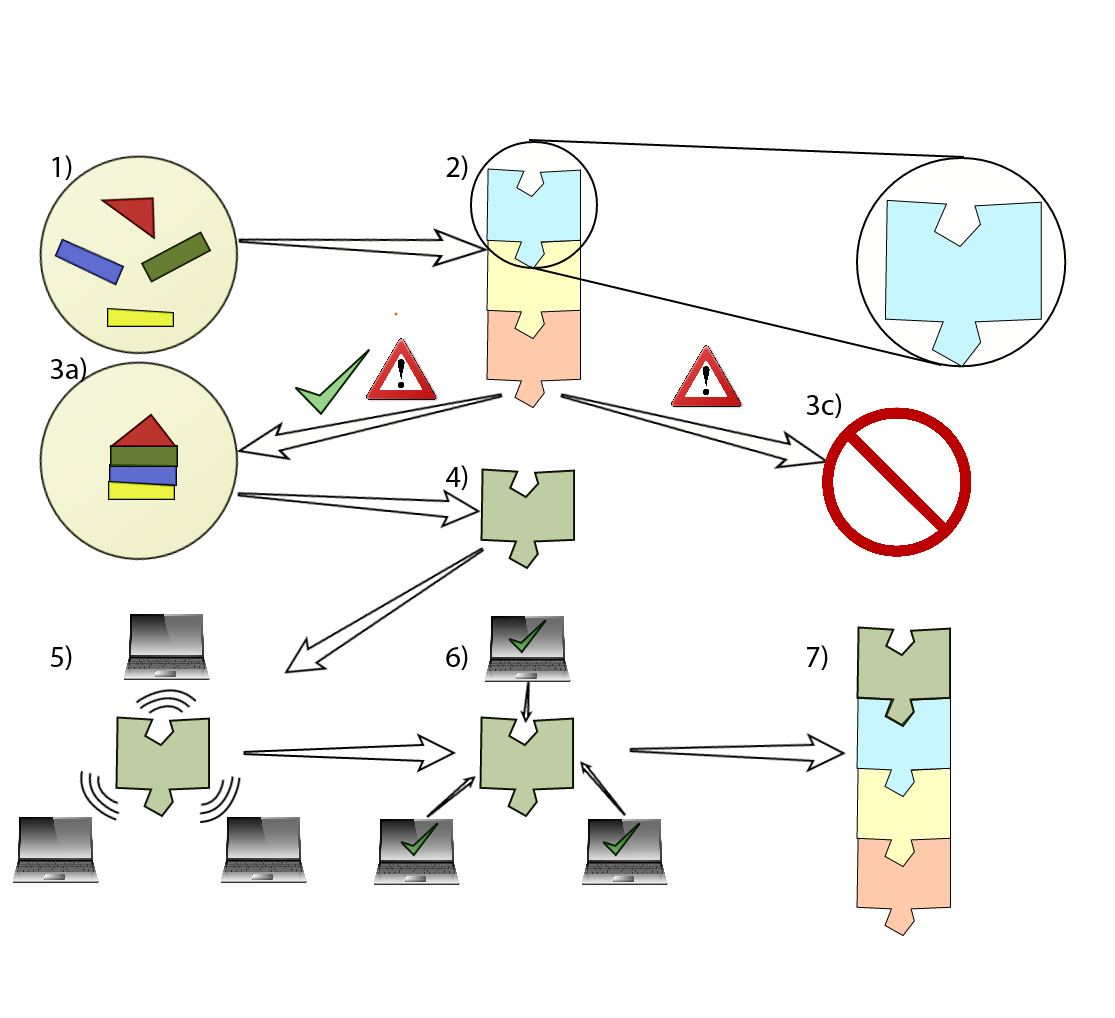
\includegraphics[width=0.6\paperwidth]{Workflow2}
	\caption{Main Workflow}
	\label{fig:main_workflow}
\end{figure}

\begin{figure}
	\centering
		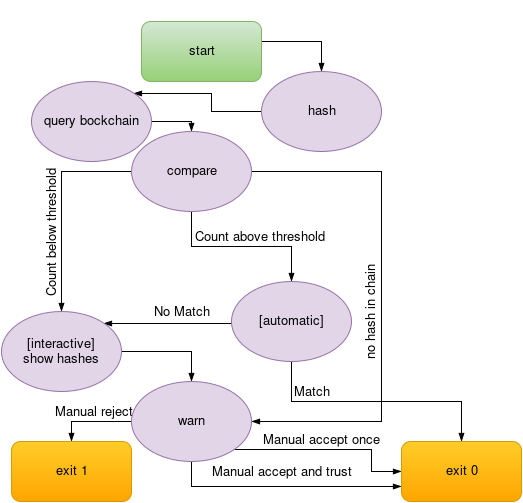
\includegraphics[width=0.45\paperwidth]{workflow}
	\caption{Decision Workflow}
	\label{fig:decision_workflow}
\end{figure}


\begin{enumerate}
	\item First of all a \textit{PKGBUILD} is downloaded and partially executed in a sandbox in order to get the package version. Then, it and any VCS sources are hashed.
	\item The resulting local hash is compared with the current consensus hash on the blockchain. [Figure \ref{fig:decision_workflow}].
	\item Now the workflow splits into 3 different paths:
	\begin{enumerate}
		\item The hashes match and the number of commits is over the threshold or the user decides to trust the locally generated hash anyway. \textit{(Followed by step 4.)} The package may be created and installed.
		\item The hashes do not match and/or the number is below the threshold, but the user wants to create and install the package without comitting the hash. \textit{(End of the workflow.)}
		The package may be created and installed.
		\item The hashes do not match and/or the number is below the threshold and the user doesn't want to create the package. \textit{(End of the workflow.)} Our program exits with a non-zero status, so an AUR helper using it would cancel the package installation at this point.
	\end{enumerate}
	\item The local hash is committed to the blockchain (this is a transaction).
	\item All nodes of the blockchain-network get the transaction.
	\item The transaction is contained in the next mined block.
	\item The block is added to the blockchain.
\end{enumerate}
